\documentclass[11pt]{article}
\usepackage[utf8]{inputenc}
\usepackage[T1]{fontenc}
\usepackage{pgfplots}
\usepackage{graphicx}
\usepackage{booktabs}
\pgfplotsset{compat=1.18}

\begin{document}

%% =====================================================================
%% Figure 1: dataset originale, x86 vs x64
%% =====================================================================
\begin{figure}[htbp]
\centering
\scalebox{0.95}{
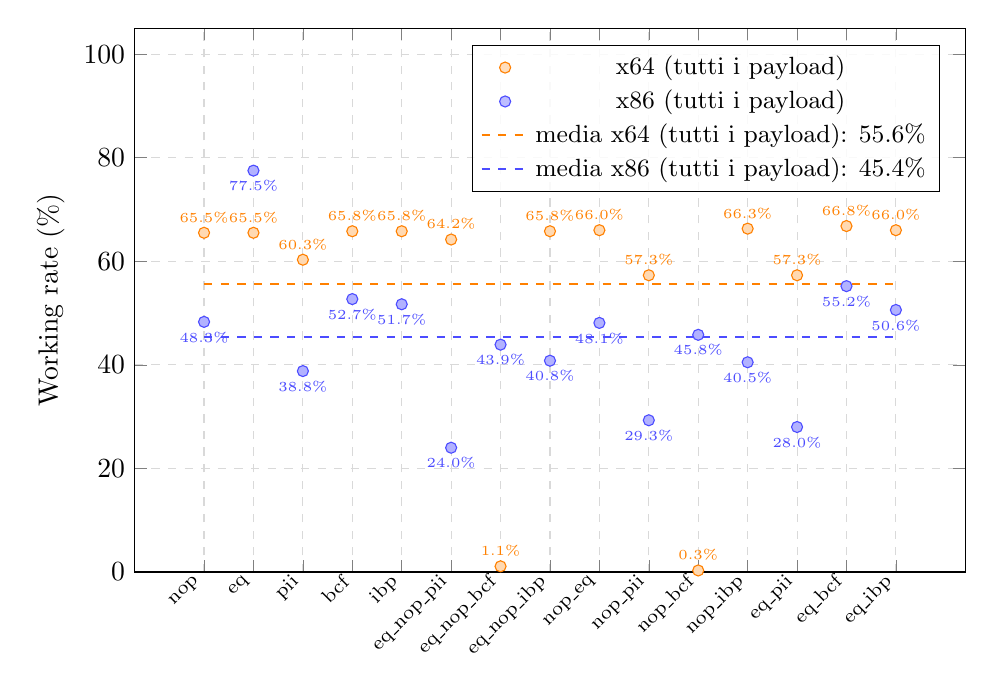
\begin{tikzpicture}
\begin{axis}[
    width=\linewidth,
    height=0.7\linewidth,
    ylabel={Working rate (\%)},
    ymin=0, ymax=105,
    ytick={0,20,40,60,80,100},
    xtick={0,...,14},
    xticklabels={nop, eq, pii, bcf, ibp, eq\_nop\_pii, eq\_nop\_bcf, eq\_nop\_ibp, nop\_eq, nop\_pii, nop\_bcf, nop\_ibp, eq\_pii, eq\_bcf, eq\_ibp},
    xticklabel style={rotate=45, anchor=east, font=\scriptsize},
    legend pos=north east,
    legend style={
        font=\small,
        fill=white,
        fill opacity=0.85,
        draw opacity=1,
        text opacity=1
    },
    grid=major,
    grid style={dashed, gray!30},
    ymajorgrids=true,
]
% medie (sotto i punti)
\addplot[orange, dashed, thick, no marks, forget plot] coordinates {(0,55.6) (14,55.6)};
\addplot[blue!70, dashed, thick, no marks, forget plot] coordinates {(0,45.4) (14,45.4)};

\addplot[only marks, mark=*, mark size=2pt, draw=orange, mark options={fill=orange!30}]
    coordinates {(0,65.5) (1,65.5) (2,60.3) (3,65.8) (4,65.8) (5,64.2) (6,1.1) (7,65.8) (8,66.0) (9,57.3) (10,0.3) (11,66.3) (12,57.3) (13,66.8) (14,66.0)};
\addlegendentry{x64 (tutti i payload)}

\addplot[only marks, mark=*, mark size=2pt, draw=blue!70, mark options={fill=blue!30}]
    coordinates {(0,48.3) (1,77.5) (2,38.8) (3,52.7) (4,51.7) (5,24.0) (6,43.9) (7,40.8) (8,48.1) (9,29.3) (10,45.8) (11,40.5) (12,28.0) (13,55.2) (14,50.6)};
\addlegendentry{x86 (tutti i payload)}

\addlegendimage{orange, dashed, thick}
\addlegendentry{media x64 (tutti i payload): 55.6\%}
\addlegendimage{blue!70, dashed, thick}
\addlegendentry{media x86 (tutti i payload): 45.4\%}

\node at (axis cs:0,65.5) [above, orange, font=\tiny] {65.5\%};
\node at (axis cs:1,65.5) [above, orange, font=\tiny] {65.5\%};
\node at (axis cs:2,60.3) [above, orange, font=\tiny] {60.3\%};
\node at (axis cs:3,65.8) [above, orange, font=\tiny] {65.8\%};
\node at (axis cs:4,65.8) [above, orange, font=\tiny] {65.8\%};
\node at (axis cs:5,64.2) [above, orange, font=\tiny] {64.2\%};
\node at (axis cs:6,1.1) [above, orange, font=\tiny] {1.1\%};
\node at (axis cs:7,65.8) [above, orange, font=\tiny] {65.8\%};
\node at (axis cs:8,66.0) [above, orange, font=\tiny] {66.0\%};
\node at (axis cs:9,57.3) [above, orange, font=\tiny] {57.3\%};
\node at (axis cs:10,0.3) [above, orange, font=\tiny] {0.3\%};
\node at (axis cs:11,66.3) [above, orange, font=\tiny] {66.3\%};
\node at (axis cs:12,57.3) [above, orange, font=\tiny] {57.3\%};
\node at (axis cs:13,66.8) [above, orange, font=\tiny] {66.8\%};
\node at (axis cs:14,66.0) [above, orange, font=\tiny] {66.0\%};
\node at (axis cs:0,48.3) [below, blue!70, font=\tiny] {48.3\%};
\node at (axis cs:1,77.5) [below, blue!70, font=\tiny] {77.5\%};
\node at (axis cs:2,38.8) [below, blue!70, font=\tiny] {38.8\%};
\node at (axis cs:3,52.7) [below, blue!70, font=\tiny] {52.7\%};
\node at (axis cs:4,51.7) [below, blue!70, font=\tiny] {51.7\%};
\node at (axis cs:5,24.0) [below, blue!70, font=\tiny] {24.0\%};
\node at (axis cs:6,43.9) [below, blue!70, font=\tiny] {43.9\%};
\node at (axis cs:7,40.8) [below, blue!70, font=\tiny] {40.8\%};
\node at (axis cs:8,48.1) [below, blue!70, font=\tiny] {48.1\%};
\node at (axis cs:9,29.3) [below, blue!70, font=\tiny] {29.3\%};
\node at (axis cs:10,45.8) [below, blue!70, font=\tiny] {45.8\%};
\node at (axis cs:11,40.5) [below, blue!70, font=\tiny] {40.5\%};
\node at (axis cs:12,28.0) [below, blue!70, font=\tiny] {28.0\%};
\node at (axis cs:13,55.2) [below, blue!70, font=\tiny] {55.2\%};
\node at (axis cs:14,50.6) [below, blue!70, font=\tiny] {50.6\%};
\end{axis}
\end{tikzpicture}
}
\caption{Working Rate Comparison (x86 vs x64), dataset originale
         \texttt{test\_report.txt}.}
\label{fig:working_rate_original}
\end{figure}

%% =====================================================================
%% Figure 2: 13 payload x64, prima vs dopo la fix getpc
%% =====================================================================
\begin{figure}[htbp]
\centering
\scalebox{0.95}{
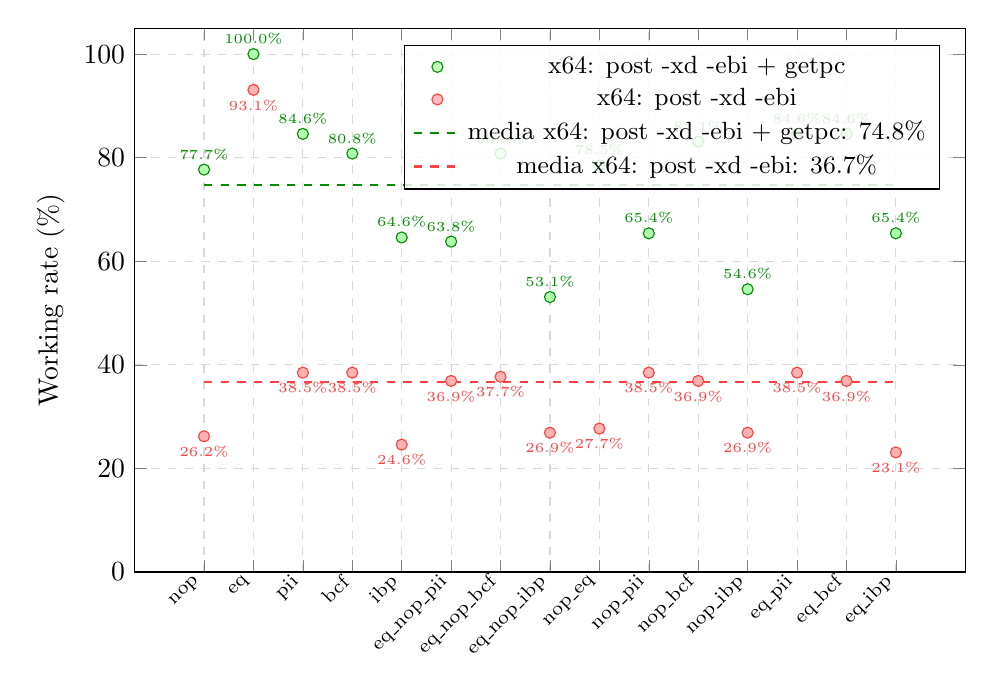
\begin{tikzpicture}
\begin{axis}[
    width=\linewidth,
    height=0.7\linewidth,
    ylabel={Working rate (\%)},
    ymin=0, ymax=105,
    ytick={0,20,40,60,80,100},
    xtick={0,...,14},
    xticklabels={nop, eq, pii, bcf, ibp, eq\_nop\_pii, eq\_nop\_bcf, eq\_nop\_ibp, nop\_eq, nop\_pii, nop\_bcf, nop\_ibp, eq\_pii, eq\_bcf, eq\_ibp},
    xticklabel style={rotate=45, anchor=east, font=\scriptsize},
    legend pos=north east,
    legend style={
        font=\small,
        fill=white,
        fill opacity=0.85,
        draw opacity=1,
        text opacity=1
    },
    grid=major,
    grid style={dashed, gray!30},
    ymajorgrids=true,
]
% medie (sotto i punti)
\addplot[green!55!black, dashed, thick, no marks, forget plot] coordinates {(0,74.8) (14,74.8)};
\addplot[red!75, dashed, thick, no marks, forget plot] coordinates {(0,36.7) (14,36.7)};

\addplot[only marks, mark=*, mark size=2pt, draw=green!55!black, mark options={fill=green!30}]
    coordinates {(0,77.7) (1,100.0) (2,84.6) (3,80.8) (4,64.6) (5,63.8) (6,80.8) (7,53.1) (8,78.5) (9,65.4) (10,83.1) (11,54.6) (12,84.6) (13,84.6) (14,65.4)};
\addlegendentry{x64: post -xd -ebi + getpc}

\addplot[only marks, mark=*, mark size=2pt, draw=red!75, mark options={fill=red!30}]
    coordinates {(0,26.2) (1,93.1) (2,38.5) (3,38.5) (4,24.6) (5,36.9) (6,37.7) (7,26.9) (8,27.7) (9,38.5) (10,36.9) (11,26.9) (12,38.5) (13,36.9) (14,23.1)};
\addlegendentry{x64: post -xd -ebi}

\addlegendimage{green!55!black, dashed, thick}
\addlegendentry{media x64: post -xd -ebi + getpc: 74.8\%}
\addlegendimage{red!75, dashed, thick}
\addlegendentry{media x64: post -xd -ebi: 36.7\%}

\node at (axis cs:0,77.7) [above, green!55!black, font=\tiny] {77.7\%};
\node at (axis cs:1,100.0) [above, green!55!black, font=\tiny] {100.0\%};
\node at (axis cs:2,84.6) [above, green!55!black, font=\tiny] {84.6\%};
\node at (axis cs:3,80.8) [above, green!55!black, font=\tiny] {80.8\%};
\node at (axis cs:4,64.6) [above, green!55!black, font=\tiny] {64.6\%};
\node at (axis cs:5,63.8) [above, green!55!black, font=\tiny] {63.8\%};
\node at (axis cs:6,80.8) [above, green!55!black, font=\tiny] {80.8\%};
\node at (axis cs:7,53.1) [above, green!55!black, font=\tiny] {53.1\%};
\node at (axis cs:8,78.5) [above, green!55!black, font=\tiny] {78.5\%};
\node at (axis cs:9,65.4) [above, green!55!black, font=\tiny] {65.4\%};
\node at (axis cs:10,83.1) [above, green!55!black, font=\tiny] {83.1\%};
\node at (axis cs:11,54.6) [above, green!55!black, font=\tiny] {54.6\%};
\node at (axis cs:12,84.6) [above, green!55!black, font=\tiny] {84.6\%};
\node at (axis cs:13,84.6) [above, green!55!black, font=\tiny] {84.6\%};
\node at (axis cs:14,65.4) [above, green!55!black, font=\tiny] {65.4\%};
\node at (axis cs:0,26.2) [below, red!75, font=\tiny] {26.2\%};
\node at (axis cs:1,93.1) [below, red!75, font=\tiny] {93.1\%};
\node at (axis cs:2,38.5) [below, red!75, font=\tiny] {38.5\%};
\node at (axis cs:3,38.5) [below, red!75, font=\tiny] {38.5\%};
\node at (axis cs:4,24.6) [below, red!75, font=\tiny] {24.6\%};
\node at (axis cs:5,36.9) [below, red!75, font=\tiny] {36.9\%};
\node at (axis cs:6,37.7) [below, red!75, font=\tiny] {37.7\%};
\node at (axis cs:7,26.9) [below, red!75, font=\tiny] {26.9\%};
\node at (axis cs:8,27.7) [below, red!75, font=\tiny] {27.7\%};
\node at (axis cs:9,38.5) [below, red!75, font=\tiny] {38.5\%};
\node at (axis cs:10,36.9) [below, red!75, font=\tiny] {36.9\%};
\node at (axis cs:11,26.9) [below, red!75, font=\tiny] {26.9\%};
\node at (axis cs:12,38.5) [below, red!75, font=\tiny] {38.5\%};
\node at (axis cs:13,36.9) [below, red!75, font=\tiny] {36.9\%};
\node at (axis cs:14,23.1) [below, red!75, font=\tiny] {23.1\%};
\end{axis}
\end{tikzpicture}
}
\caption{Working rate x64 sui 13 payload a basso rate: confronto tra il run
         \texttt{-xd -ebi} e il run \texttt{-xd -ebi} + fix getpc.}
\label{fig:working_rate_getpc}
\end{figure}

%% =====================================================================
%% Tabella riassuntiva per payload
%% =====================================================================
\begin{table}[htbp]
\centering
\small
\caption{Working rate per payload (13 payload x64). \emph{Originale} = nessun
         flag; \emph{Post \texttt{-xd -ebi}} = capstone 5.0.0.post1 con
         \texttt{-xd -ebi} (prima della fix getpc); \emph{Post \texttt{-xd -ebi}
         + getpc} = run aggiornato. Tra parentesi OK/test.}
\label{tab:working_rate_payloads}
\begin{tabular}{lrrrr}
\toprule
Payload & Originale & Post \texttt{-xd -ebi} & Post \texttt{-xd -ebi} + getpc & $\Delta$ \\
\midrule
\texttt{windows\_x64\_custom\_reverse\_https} & 0.0 (0/149) & 94.0 (141/150) & 88.0 (132/150) & -6.0 \\
\texttt{windows\_x64\_custom\_reverse\_winhttp} & 0.0 (0/149) & 6.7 (10/150) & 93.3 (140/150) & +86.6 \\
\texttt{windows\_x64\_custom\_reverse\_winhttps} & 0.0 (0/150) & 6.7 (10/150) & 6.7 (10/150) & +0.0 \\
\texttt{windows\_x64\_meterpreter\_reverse\_http} & 0.0 (0/149) & 4.7 (7/150) & 88.7 (133/150) & +84.0 \\
\texttt{windows\_x64\_meterpreter\_reverse\_https} & 0.0 (0/149) & 6.7 (10/150) & 88.0 (132/150) & +81.3 \\
\texttt{windows\_x64\_meterpreter\_reverse\_winhttp} & 0.0 (0/149) & 82.0 (123/150) & 88.0 (132/150) & +6.0 \\
\texttt{windows\_x64\_vncinject\_reverse\_http} & 0.0 (0/150) & 2.7 (4/150) & 89.3 (134/150) & +86.6 \\
\texttt{windows\_x64\_vncinject\_reverse\_winhttp} & 0.0 (0/150) & 6.7 (10/150) & 92.7 (139/150) & +86.0 \\
\texttt{windows\_x64\_vncinject\_reverse\_winhttps} & 0.0 (0/150) & 6.7 (10/150) & 6.7 (10/150) & +0.0 \\
\texttt{windows\_x64\_meterpreter\_reverse\_winhttps} & 1.3 (2/150) & 82.7 (124/150) & 76.7 (115/150) & -6.0 \\
\texttt{windows\_x64\_vncinject\_reverse\_https} & 1.3 (2/149) & 6.7 (10/150) & 94.7 (142/150) & +88.0 \\
\texttt{windows\_x64\_messagebox} & 2.7 (4/150) & 73.3 (110/150) & 72.0 (108/150) & -1.3 \\
\texttt{windows\_x64\_custom\_reverse\_http} & 10.2 (15/147) & 98.0 (147/150) & 87.3 (131/150) & -10.7 \\
\midrule
\textbf{Totale (13)} & 1.2 (23/1941) & 36.7 (716/1950) & 74.8 (1458/1950) & +38.1 \\
\bottomrule
\end{tabular}
\end{table}

\end{document}
